% !TeX root = ../../book.tex
\section{单射与满射}
\secbegin{secInjectionsSurjections}
\index{injection|(}
\index{surjection|(}
\index{bijection|(}

为了引出某些定义，我们先来做个实验。请观察下面的点 ($\bullet$) 和星 ($\star$)。是点更多还是星更多？
\begin{center}
\fitwidth{\begin{tikzpicture}
\foreach \x in {1,2,3,4,5,6,7,8,9,10,11,12,13,14,15,16,17,18,19}
  \node at (0.75*\x, 0.75) {$\bullet$};

\foreach \x in {1,2,3,4,5,6,7,8,9,10,11,12,13,14,15}
  \node at (0.75*\x, 0) {$\star$};
\end{tikzpicture}}
\end{center}

暂停一下，想一想你是如何知道这个问题的答案的。

答案是，点比星多。有几种方法可以得出此结论：
\begin{enumerate}[(i)] 
\item 你可以数一下点的数量，再数一下星的数量，然后比较这两个数字哪个大；
\item 你可能会注意到，点和星间隔均匀，但点的队列比星的队列长。
\end{enumerate}
你很可能使用了方法(ii)。事实上，你可能从未数过点的数量或星的数量 --- 而且也不需要！通过简单地将点与星配对，我们可以得出结论，点比星多 --- 我们最终用完了所有的星，但仍然剩下点，所以点一定比星多。

\subsection*{单射}

将星与点在数学上配对的行为可以用函数形式化，定义 $f : S \to D$ 为从星集 $S$ 到点集 $D$ 的函数，其中每颗星的 $f$ 值都是与其配对的点。当然，我们必须以满足：每个点最多与一颗星星配对：

\begin{center}
\fitwidth{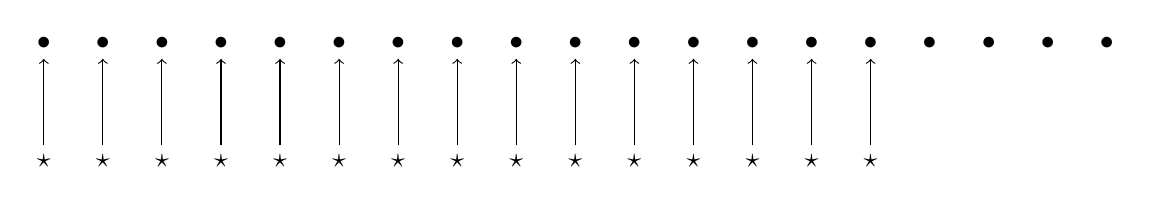
\begin{tikzpicture}
\foreach \x in {1,2,3,4,5,6,7,8,9,10,11,12,13,14,15,16,17,18,19}
  \node at (0.75*\x, 1.5) {$\bullet$};

\foreach \x in {1,2,3,4,5,6,7,8,9,10,11,12,13,14,15}
  \node at (0.75*\x, 0) {$\star$};

\foreach \x in {1,2,3,4,5,6,7,8,9,10,11,12,13,14,15}
  \draw [->] (0.75*\x, 0.2) -- (0.75*\x, 1.3);
\end{tikzpicture}}
\end{center}

函数的这一属性 --- 称为 \textit{单射} --- 让我们能够推断出点的数量多于星的数量。

直观地说，如果函数 $f : X \to Y$ 将 $X$ 的元素与 $Y$ 子集的元素一一对应，那么它就是单射的 --- 就像上例中星与点的子集一一对应一样。

\begin{definition}
\label{defInjective}\label{defInjection}
\index{function!injective (one-to-one)}
\index{injection}
如果函数 $f : X \to Y$ 满足于
\[ \forall a,b \in X,\, f(a) = f(b) \Rightarrow a=b \]
则说 $f$ 是 \textbf{单射的} (或 \textbf{一对一的})。
单射的函数被称为\textbf{单射}。
\end{definition}

\begin{strategy}[证明函数是单射的]
要想证明函数 $f : X \to Y$ 是单射的，只需给定 $a,b \in X$，假设 $f(a)=f(b)$，然后推导出 $a=b$。
\end{strategy}

反过来，$f : X \to Y$ 是单射的，相当于说，对于所有 $a,b \in X$，如果 $a \ne b$，则 $f(a) \ne f(b)$ 。这点通常对\textit{证明}函数是单射的没什么用，但它确实提供了很好的直觉 --- 它表示 $f$ 将不同的输入匹配到不同的输出。

下面是一个非常简单的初等算术示例：
\begin{example}
定义函数 $f : \mathbb{Z} \to \mathbb{Z}$ 为对于所有 $n \in \mathbb{Z}$, $f(x) = 2n+1$。证明 $f$ 是单射的。给定 $m, n \in \mathbb{Z}$，并假设 $f(m)=f(n)$。根据 $f$ 的定义，我们有 $2m+1=2n+1$。两边同时减 $1$ 得 $2m=2n$，两边同时除以 $2$ 得 $m=n$。因此 $f$ 是单射的。
\end{example}

下面的示例稍微复杂一些。

\begin{proposition}
\label{propCompositeOfInjectionsIsInjection}
设 $f : X \to Y$ 和 $g : Y \to Z$ 为函数。如果 $f$ 和 $g$ 都是单射的，则 $g \circ f$ 也是单射的。
\end{proposition}
\begin{cproof}
假设 $f$ 和 $g$ 都是单射的且
%% BEGIN EXTRACT (xtrVariableIntroductionExample) %%
设 $a,b \in X$。
我们要证明
\[ (g \circ f)(a) = (g \circ f)(b) \quad \Rightarrow \quad a=b \]
%% END EXTRACT %%
假设 $(g \circ f)(a) = (g \circ f)(b)$。根据函数组合的定义，这意味着 $g(f(a))=g(f(b))$。因为 $g$ 是单射的，我们有 $f(a)=f(b)$；又因为 $f$ 是单射的，我们有 $a=b$。
\end{cproof}

\begin{exercise}
设 $f : X \to Y$ 和 $g : Y \to Z$ 为函数。证明如果 $g \circ f$ 是单射的，则 $f$ 是单射的。
\end{exercise}

\begin{exercise}
写出函数 $f : X \to Y$ \textit{不是}单射的含义，并说明如何证明给定函数不是单射的。给出一个非单射函数的例子，并给出它不是单射的证明。
\end{exercise}

\begin{exercise}
判断下列函数是否是单射的。
\begin{itemize} 
\item $f : \mathbb{N} \to \mathbb{Z}$，定义为对于所有 $n \in \mathbb{N}$, $f(n)=n^2$。
\item $g : \mathbb{Z} \to \mathbb{N}$，定义为对于所有 $n \in \mathbb{Z}$, $g(n)=n^2$。
\item $h : \mathbb{N} \times \mathbb{N} \times \mathbb{N} \to \mathbb{N}$，定义为对于所有 $x,y,z \in \mathbb{N}$, $h(x,y,z) = 2^x \cdot 3^y \cdot 5^z$。
\end{itemize}
\end{exercise}

\begin{exercise}
\label{exLinearPolynomialIsInjective}
设 $a,b \in \mathbb{R}$ 且 $b \ne 0$，定义函数 $f : \mathbb{R} \to \mathbb{R}$ 为对于所有$t \in \mathbb{R}$, $f(t) = a+bt$。证明 $f$ 是单射的。
\end{exercise}

\subsection*{满射}

让我们回顾一下之前看到的一排点和星。之前，我们通过证明从星集 $S$ 到点集 $D$ 存在单射 $f : S \to D$，正式提出了点比星更多的想法。

然而，我们可以通过定义函数 $D \to S$ 得出相同的结论，它在某种意义上意味着点\textit{涵盖}星 --- 也就是说，每个星都至少与一个点配对。

\begin{center}
\fitwidth{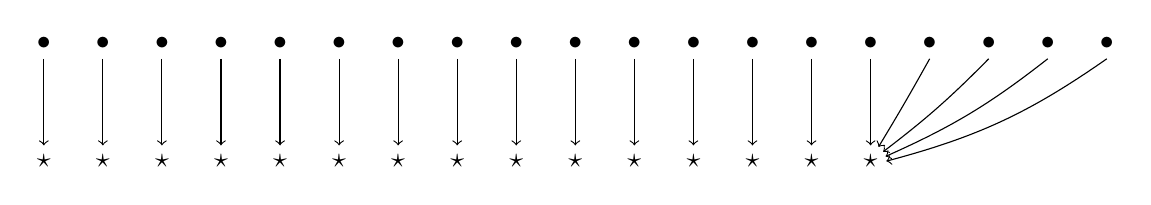
\begin{tikzpicture}
\foreach \x in {1,2,3,4,5,6,7,8,9,10,11,12,13,14,15,16,17,18,19}
  \node at (0.75*\x, 1.5) {$\bullet$};

\foreach \x in {1,2,3,4,5,6,7,8,9,10,11,12,13,14,15}
  \draw [->] (0.75*\x, 1.3) -- (0.75*\x, 0.2);

  \draw [->] (12, 1.3) to [bend left=1] (11.35, 0.18);
  \draw [->] (12.75, 1.3) to [bend left=4] (11.41, 0.12);
  \draw [->] (13.5, 1.3) to [bend left=7] (11.44, 0.06);
  \draw [->] (14.25, 1.3) to [bend left=10] (11.45, 0);

\foreach \x in {1,2,3,4,5,6,7,8,9,10,11,12,13,14,15}
  \node at (0.75*\x, 0) {$\star$};
\end{tikzpicture}}
\end{center}

这个性质称为\textit{满射性} --- 如果 $Y$ 的每个元素都是 $f$ 的值，则函数 $f : X \to Y$ 是满射的。\Cref{defSurjective} 对此进行了精确说明。

\begin{definition}
\label{defSurjective}\label{defSurjection}
如果函数 $f : X \to Y$ 满足
\[ \forall y \in Y,\ \exists x \in X,\ f(x) = y \]
则说 $f$ 是 \textbf{满射的}\index{function!surjective}\index{surjection} (或 \textbf{onto})。
满射的函数被称为\textbf{满射}。
\end{definition}

\begin{strategy}
要证明函数 $f : X \to Y$ 是满射的，只需取任意元素 $y \in Y$ 并根据 $y$ 找到元素 $x \in X$ 满足 $f(x)=y$ 即可。

为了找到$x$，通常会从方程 $f(x)=y$ 开始并推导出 $x$ 的可能值。但要小心 --- 为了完成证明，有必要验证方程 $f(x)=y$ 对于所选的 $x$ 值是否成立。
\end{strategy}

\begin{example}
给定 $n \in \mathbb{N}$ 且 $n > 0$，并定义函数 $r : \mathbb{Z} \to \{ 0, 1, \dots, n-1 \}$ 为 $r(a)$ 是 $a$ 除以 $n$ 的余数 (见 \Cref{thmDivisionPreliminary})。这个函数是满射的，因为对于每个 $k \in \{ 0, 1, \dots, n-1 \}$，我们有 $r(k)=k$。
\end{example}

\begin{exercise}
对于以下每一个集合对 $(X,Y)$，判断由 $f(x)=2x+1$ 定义的函数 $f : X \to Y$ 是否是满射。
\begin{enumerate}[(a)]
\item $X = \mathbb{Z}$ 且 $Y = \{ x \in \mathbb{Z} \mid x \text{ 为奇数} \}$;
\item $X = \mathbb{Z}$ 且 $Y = \mathbb{Z}$;
\item $X = \mathbb{Q}$ 且 $Y = \mathbb{Q}$;
\item $X = \mathbb{R}$ 且 $Y = \mathbb{R}$.
\end{enumerate}
\end{exercise}

\begin{exercise}
设 $f : X \to Y$ 为函数。找到子集 $V \subseteq Y$ 和满射 $g : X \to V$ 满足 $f$（也就是说，对于所有 $x \in X$, $g(x)=f(x)$）。
\hintlabel{exSurjectiveCorestriction}{%
回想一下\Cref{defImage}。
}
\end{exercise}

\begin{exercise}
设 $f : X \to Y$ 为函数。证明 $f$ 是满射的当且仅当 $Y=f[X]$
\end{exercise}

\begin{exercise}
\label{exEpiMonoFactorisation}
设 $f : X \to Y$ 为函数。证明存在集合 $Z$ 和函数
\[ p : X \to Z \quad \text{和} \quad i : Z \to Y \]
使得 $p$ 是满射的，$i$ 是单射的，且 $f = i \circ p$。
\begin{backhint}
\hintref{exEpiMonoFactorisation}
如果 $Z$ 是 $Y$ 的子集，那么对于所有 $z \in Z$ 我们可以很容易地定义一个单射 $i : Z\to Y$。是否存在 $Y$ 的子集与值域为$Y$ 的函数关联？
\end{backhint}
\end{exercise}

\begin{exercise}
设 $f : X \to \mathcal{P}(X)$ 为函数。通过考虑集合 $B = \{ x \in X \mid x \not\in f(x) \}$，证明 $f$ 不是满射的。
\hintlabel{exRussellSubset}{%
注意 $B \in \mathcal{P}(X)$。 证明不存在 $a \in X$ 使得 $B = f(a)$。
}
\end{exercise}

\subsection*{双射}

双射函数形式化了将集合一一对应的思想 --- 集合中的每个元素都与另一集合中的唯一一个元素配对。

\begin{definition}
\label{defBijective}\label{defBijection}
如果函数 $f : X \to Y$ 即是单射的又是满射的，则它是\textbf{双射的}\index{function!bijective} 。双射的函数被称为\textbf{双射}\index{bijection}.
\end{definition}

\begin{prooftip}
要证明函数 $f$ 是双射的，只需证明它即是单射的又是满射的。
\end{prooftip}

\begin{example}
\label{exDyadicRationalsBijection}
设 $D \subseteq \mathbb{Q}$ 为\textit{二进有理数}集，即
\[ D = \left\{ x \in \mathbb{Q} \ \bigg|\  x = \frac{a}{2^n} \text{ for some } a \in \mathbb{Z} \text{ and } n \in \mathbb{N} \right\} \]
设 $k \in \mathbb{N}$，并由定义函数 $f : D \to D$ 为 $f(x)=\frac{x}{2^k}$。证明 $f$ 是双射。
\begin{itemize}
\item (\textbf{单射性}) 给定 $x,y \in D$ 且假设 $f(x)=f(y)$。则 $\frac{x}{2^k}=\frac{y}{2^k}$，因此 $x=y$。
\item (\textbf{满射性}) 给定 $y \in D$。我们需要找到 $x \in D$ 使得 $f(x)=y$。很明显如果 $2^ky \in D$ 则我们有 \[ f(2^ky)=\frac{2^ky}{2^k}=y \]
因此只需证明 $2^ky \in D$ 即可。
%% BEGIN EXTRACT (xtrCasesExample)
因为 $y \in D$，必有对于某个 $n \in \mathbb{N}$, $y=\frac{a}{2^n}$。
\begin{itemize}
\item 如果 $k \le n$ 则 $n-k \in \mathbb{N}$，因此 $2^ky=\frac{a}{2^{n-k}} \in D$。
\item 如果 $k > n$ 则 $k-n>0$ 且 $2^ky = 2^{k-n}a \in \mathbb{Z}$；因为如果 $a \in \mathbb{Z}$ 则 $a=\frac{a}{2^0}$，所以 $\mathbb{Z} \subseteq D$。因此我们再一次得到 $2^ky \in D$。
\end{itemize}
综上两种情况我们得到 $2^ky \in D$；且 $f(2^ky)=y$，因此 $f$ 是满射的。
%% END EXTRACT
\end{itemize}
因为 $f$ 既是单射的又是满射的，所以它是双射的。
\end{example}

\begin{exercise}
\label{exIdentityBijection}
设 $X$ 为集合。证明恒等函数 $\mathrm{id}_X : X \to X$ 是双射。
\end{exercise}

\begin{exercise}
\label{exCompositeOfBijectionsIsBijection}
设 $f : X \to Y$ 和 $g : Y \to Z$ 为双射。证明 $g \circ f$ 也是双射。
\end{exercise}

\subsection*{反函数}

我们的下一个目标是用被称为\textit{反函数}的函数来表征单射、满射和双射。

回想一下 \Cref{defInjection}，它表示函数 $f : X \to Y$ 如果对于所有 $a,b \in X$，可以得到 $f(a)=f(b)$ 则 $a=b$，那么函数是单射的。

\begin{exercise}
设 $f : X \to Y$ 为函数。证明 $f$ 是单射的当且仅当
\[ \forall y \in f[X],\, \exists ! x \in X,\, y=f(x) \]
\end{exercise}

回想 \Cref{secFunctions}，你可能会注意到这意味着逻辑公式 `$y=f(x)$' 定义了一个函数 $f[X] \to X$ --- 具体来说，如果 $f$ 是单射的，那么有一个函数 $g : f[X] \to X$ ，它是通过为所有 $x \in X$ 指定 $x=g(f(x))$ 来（明确）定义的。将 $f$ 视为\textit{编码}函数，则 $g$ 是相应的\textit{解码}函数 --- 通过 $f$ 的单射性可以进行解码。（如果 $f$ 不是单射的，那么 $X$ 的不同元素可能具有相同的编码，在这种情况下，如果我们尝试解码它们，我们就会陷入困境！）

\begin{exercise}
\label{exEncodingPairs}
定义函数 $e : \mathbb{N} \times \mathbb{N} \to \mathbb{N}$ 为 $e(m,n) = 2^m \cdot 3^n$。证明 $e$ 是单射的。我们可以将 $e$ 视为将自然数\textit{对}编码为单个自然数 --- 例如，自然数对 $(4,1)$ 编码为 $2^4 \cdot 3^1 = 48$。对于以下每个自然数 $k$，找到由 $e$ 编码为 $k$ 的自然数对：
\[ 1 \qquad 24 \qquad 7776 \qquad 59049 \qquad 396718580736 \]
\end{exercise}

在 \Cref{exEncodingPairs} 中，我们能够将 $2^m \cdot 3^n$ 形式的任何自然数解码为 $m,n \in \mathbb{N}$。这个解码过程产生一个函数
\[ d : \{ k \in \mathbb{N} \mid k=2^m \cdot 3^n \text{ 对某个 } m,n \in \mathbb{N} \} \to \mathbb{N} \times \mathbb{N} \]
如果我们尝试解码一个不是 $2^m \cdot 3^n$ 形式的自然数为 $m,n \in \mathbb{N}$，比如 $5$ 或 $100$，会发生什么？好吧\dots{}这并不重要！重要的是对于所有 $(m,n) \in \mathbb{N} \times \mathbb{N}$, $d(e(m,n))=(m,n)$ 成立；$d$ 对其他自然数的值是无关的。

\begin{definition}
\label{defLeftInverse}
\index{inverse!left inverse}
\index{left inverse}
设 $f : X \to Y$ 为函数。$f$ 的\textbf{左逆}（或\textbf{后逆}）为函数 $g : Y \to X$，满足 $g \circ f = \mathrm{id}_X$。
\end{definition}

\begin{example}
设 $e : \mathbb{N} \times \mathbb{N} \to \mathbb{N}$ 与 \Cref{exEncodingPairs} 中定义的函数一样。定义函数 $d : \mathbb{N} \to \mathbb{N} \times \mathbb{N}$ 为
\[ d(k) = \begin{cases}
(m,n) & \text{if } k=2^m \cdot 3^n \text{ for some } m,n \in \mathbb{N} \\
(0,0) & \text{otherwise}
\end{cases} \]
请注意，$d$ 是由算术基本定理 (\Cref{thmFTA}) 明确定义的。此外，给定 $m,n \in \mathbb{N}$，我们有
\[ d(e(m,n)) = d(2^m \cdot 3^n) = (m,n) \]
所以 $d$ 是 $e$ 的左逆。
\end{example}

\begin{exercise}
\label{exIfHasLeftInverseThenInjective}
设 $f : X \to Y$ 为函数。证明如果 $f$ 存在左逆，则 $f$ 是单射的。
\end{exercise}

\Cref{exIfHasLeftInverseThenInjective} 为我们提供了一种证明函数为单射的新策略。

\begin{strategy}[通过左逆证明函数为单射]
要想证明函数 $f : X \to Y$ 是单射的，只需找到函数 $g : Y \to X$ 对于所有 $x \in X$ 满足 $g(f(x)) = x$ 即可。
\end{strategy}

如果 \Cref{exIfHasLeftInverseThenInjective} 的逆命题为真，那就方便多了 --- 而且确实如此，只要我们强加一个条件，即函数的定义域非空。

\begin{proposition}
\label{propIfInjectiveThenHasLeftInverse}
设 $f : X \to Y$ 为函数。如果 $f$ 为单射的且 $X$ 非空，则 $f$ 有一个左逆。
\end{proposition}

\begin{cproof}
假设 $f$ 是单射的且 $X$ 非空。给定 Fix $x_0 \in X$ --- 请注意，该元素存在是因为 $X$ 非空 --- 并定义 $g : Y \to X$ 为
\[ g(y) = \begin{cases} x & \text{如果 } y=f(x) \text{ 对于某个 } x \in X \\ x_0 & \text{否则} \end{cases} \]
$g$ 定义中唯一可能导致其无法明确定义的部分是当 $y=f(x)$ 对于某个 $x \in X$ 时的情况。$g$ 明确良好的原因正是 $f$ 的单射性：如果 $y=f(x)$ 对于某个 $x \in X$，则 $x \in X$ 的值对于 $y = f(x)$ 是唯一的。（事实上，如果 $a \in X$ 满足 $y=f(a)$，那么我们通过 $f$ 的单射性可得 $a=x$。）

所以 $g$ 确实是明确定义的。要证明 $g$ 是 $f$ 的左逆，设 $x \in X$。设 $y = f(x)$，我们看到 $y$ 属于 $g$ 定义中的第一种情况，因此对于值 $a \in X$ 有 $g(f(x)) = g(y) = a$，其中 $y = f(a)$ --- 如上所述，通过 $f$ 的单射性我们有 $a=x$。
\end{cproof}

\begin{exercise}
设 $f : X \to Y$ 为函数，其左逆为 $g : Y \to X$。证明 $g$ 是满射的。
\hintlabel{exLeftInversesAreSurjective}{%
这可以用一句话来证明；如果你发现自己写了一个很长的证明，那么一定有更简单的方法。
}
\end{exercise}

我们在 \Cref{exIfHasLeftInverseThenInjective,propIfInjectiveThenHasLeftInverse} 中建立了单射和左逆之间的关系，那么满射和\textit{右}逆之间存在关系也就不足为奇了。

\begin{definition}
\label{defRightInverse}
\index{inverse!right inverse}
\index{right inverse}
设 $f : X \to Y$ 为函数。$f$ 的\textbf{右逆}（或\textbf{前逆}）为函数 $g : Y \to X$，满足 $f \circ g = \mathrm{id}_Y$。
\end{definition}

\begin{example}
定义 $f : \mathbb{R} \to \mathbb{R}^{\ge 0}$ 为 $f(x)=x^2$。注意，$f$ 是满射的，因为对于每个 $y \in \mathbb{R}^{\ge 0}$ 我们有 $\sqrt{y} \in \mathbb{R}$ 且 $f(\sqrt{y}) = y$。然而 $f$ 不是单射的；例如
\[ f(-1) = 1 = f(1) \]
下面是 $f$ 的三个右逆：
\begin{itemize}
\item 正平方根函数 $g : \mathbb{R}^{\ge 0} \to \mathbb{R}$ 定义为对于所有 $y \in \mathbb{R}^{\ge 0}$, $g(y)=\sqrt{y}$。事实上，对于每个 $y \in \mathbb{R}^{\ge 0}$ 我们有
\[ f(g(y)) = f(\sqrt{y}) = (\sqrt{y})^2 = y \]
\item 负平方根函数 $h : \mathbb{R}^{\ge 0} \to \mathbb{R}$ 定义为对于所有 $y \in \mathbb{R}^{\ge 0}$, $h(y)=-\sqrt{y}$。事实上，对于每个 $y \in \mathbb{R}^{\ge 0}$ 我们有
\[ f(h(y)) = f(-\sqrt{y}) = (-\sqrt{y})^2 = y \]
\item 函数 $k : \mathbb{R}^{\ge 0} \to \mathbb{R}$ 定义为
\[ k(y) = \begin{cases}
\sqrt{y} & \text{如果 } 2n \le y < 2n+1 \text{ 对于某个 } n \in \mathbb{N} \\
-\sqrt{y} & \text{否则}
\end{cases} \]
请注意，$k$ 是明确定义的，并且对于所有 $y \in \mathbb{R}^{\ge 0}$ 来说，$f(k(y)) = y$ 依然成立，因为无论 $k(y)$ 取什么值，都等于 $\sqrt{y}$ 或 $-\sqrt{y}$。
\end{itemize}
$f$ 还有更多的右逆 --- 事实上，有无穷多个！
\end{example}

\begin{exercise}
设 $f : X \to Y$ 为函数。证明如果 $f$ 存在右逆，则 $f$ 是满射的。
\hintlabel{exIfHasRightInverseThenSurjective}{%
证明几乎与 \Cref{exLeftInversesAreSurjective} 相同。
}
\end{exercise}

\begin{strategy}[通过右逆证明函数为满射]
要想证明函数 $f : X \to Y$ 是满射的，只需找到函数 $g : Y \to X$ 对于所有 $y \in Y$ 满足 $f(g(y)) = y$ 即可。
\end{strategy}

\subsection*{插曲：选择公理}

如果 \Cref{exIfHasRightInverseThenSurjective} 的逆命题成立，那就会方便很多 --- 也就是说，如果 $f : X \to Y$ 是满射，那么它有一个右逆。让我们来看看这个事实的证明需要什么。$f : X \to Y$ 是满射可以表示为
\[ \forall y \in Y,\, \exists x \in X,\, f(x) = y \]
右逆为函数 $g : Y \to X$，根据 \Cref{defFunction}，它必满足如下条件
\[ \forall y \in Y,\, \exists ! x \in X,\, g(y) = x \]

因此，我们倾向于按如下方式构造 $g : Y \to X$。设 $y \in Y$。根据满射的定义，存在 $x \in X$，使得 $f(x) = y$ --- 定义$g(y)$ 为这样的元素 $x$。然后根据需要我们有 $f(g(y)) = f(x) = y$。

这种构造有一个极其微妙但重要的问题。

通过选择 $g(y)$ 作为 $X$ 的固定元素，使得 $f(x) = y$，我们提前假设存在一种选择机制，对于每个 $y \in Y$ ，$f^{-1}[\{y\}]$ 的唯一元素为 $g(y)$ 的值。换句话说，我们假设某个陈述 $R(x,y)$ 满足以下属性
\[ \forall y \in Y,\, \exists ! x \in X,\, [x \in f^{-1}[\{y\}] \wedge R(x,y)] \]
而根据 \Cref{defFunction}，这个假设准确地说存在一个函数 $Y \to X$，其中每个元素 $y \in Y$ 与一个元素 $x \in X$ 关联，使得 $f(x) = y$。

用更简单的术语来说：我们试图通过假设 $f$ 存在右逆来证明 $f$ 存在右逆。显然，这不是一个有效的证明策略。

令人惊讶的是，事实证明，无论是每个满射都有右逆的假设，还是存在没有右逆的满射的假设，都不会导致矛盾。因此，每个满射都有右逆的断言是\textit{不可证明的}，尽管证明它是不可证明的远远超出了本书的范畴。

然而，我们上面给出的右逆的构造并没有让人\textit{感觉}我们在滥用数学和逻辑的结构。

证明的本质是，如果 $\forall a \in A,\, \exists b \in B,\, p(a,b)$ 形式的陈述为真，那么我们应该能够定义一个函数 $h : A \to B$ 使得 $p(a,h(a))$ 对于所有 $a \in A$ 为真：函数 $h$ 为每个 $a \in A$ `选择'特定元素 $b = h(a) \in B$ 使得 $p(a,b)$ 为真。

\textit{选择公理}使其成为可能，如下所述。

\begin{axiom}[选择公理]
\label{axChoice}
\index{axiom of choice}
设 $\{ X_i \mid i \in I \}$ 为非空集族。则存在函数 $h : I \to \bigcup\limits_{i \in I} X_i$ 满足对于每个 $i \in I$, $h(i) \in X_i$。
\end{axiom}

了解选择公理是有必要的：
\begin{itemize}
\item 选择公理也许是我们所做的\textit{最奇怪}的假设 --- 我们所说的大多数其他公理都是`明显正确的'，但选择公理的情况并非如此；
\item 有些数学领域需要将关于集合的结果转换为关于其他类型对象的结果 --- 知道是否需要用到选择公理来证明结果，告诉我们是否存在这种可能性；
\item 选择公理是高度非构造性的：如果不使用选择公理也能证明结果，那它通常比使用选择公理证明相同结果提供更多信息。
\end{itemize}

考虑到这一点，当我们需要使用选择公理来证明结果时，我们会用字母 {\small \textbf{AC}} 标记结果。第一次阅读时可以忽略这一点，但读者在以后使用本书作为参考时可能会发现它很有用。

\begin{propositionac}
\label{propUsingAC}
设 $X$ 和 $Y$ 为集合并设 $p(x,y)$ 为具有自由变量 $x \in X$ 和 $y \in Y$ 的逻辑公式。如果 $\forall x \in X,\, \forall y \in Y,\, p(x,y)$ 为真，则存在函数 $h : X \to Y$ 使得 $\forall x \in X,\, p(x,h(x))$ 为真。
\end{propositionac}

\begin{cproof}
对于每个 $a \in X$，定义 $Y_a = \{ b \in Y \mid p(a,b) \}$。请注意，根据假设 $\forall x \in X,\, \exists y \in Y,\, p(x,y)$ 为真，对于每个 $a \in X$, $Y_a$ 非空。因为对于每个 $a \in X$, $Y_a \subseteq Y$，根据选择公理，存在函数 $h : X \to Y$ 使得对于所有 $a \in X$, $h(a) \in Y_a$。而根据集合 $Y_a$ 的定义，对于每个 $a \in X$, $p(a,h(a))$ 都为真。
\end{cproof}

根据 \Cref{propUsingAC}，选择公理在证明中表现为以下证明策略。

\begin{strategyac}[做出选择]
\label{strUsingAC}
如果证明中的假设具有 $\forall x \in X,\, \exists y \in Y,\, p(x,y)$ 这种形式，则我们可以对每个 $a \in A$ 做出选择，选择特性元素 $b = b_a \in B$ 使得 $p(a,b)$ 为真。
\end{strategyac}

\subsection*{回到反函数}

现在我们回到 \Cref{exIfHasRightInverseThenSurjective} 的逆命题。

\begin{propositionac}
每个满射都有一个右逆。
\end{propositionac}

\begin{cproof}
设 $f : X \to Y$ 为满射，并定义 $g : Y \to X$ 如下。给定 $y \in Y$，将 $g(y)$ 定义为 $x \in X$ 的特定选择，使得 $f(x) = y$ --- 请注意，由于 $f$ 是满射，因此存在这样一个元素 $x \in X$，因此 $g$ 存在于 \Cref{strUsingAC} 中。而根据 $g$ 的定义，对于所有 $y \in Y$，我们有 $f(g(y)) = y$，因此 $g$ 是一个满射。
\end{cproof}

我们可以将双射分类为具有左逆和右逆的函数，这似乎很合逻辑。实际上我们可以说得更强硬一些 --- 左逆和右逆可以被认为是同一函数！（事实上​​，\Cref{propLeftAndRightInversesAreEqual} 确定它们必然是相同的函数。） 

\begin{definition}
\label{defInverse}
\index{inverse!two-sided}
\index{two-sided inverse}
设 $f : X \to Y$ 为函数。$f$ 的（\textbf{双边}）\textbf{逆}为函数 $g : Y \to X$，它既是 $f$ 的左逆又是右逆。
\end{definition}

人们习惯上简单地说`逆'而不是`双边逆'。

\begin{example}
设 $D$ 为是二元有理数集，如 \Cref{exDyadicRationalsBijection} 定义。定义函数 $f : D \to D$ 为对于所有 $x \in D$, $f(x)=\frac{x}{2^k}$，其中 $k$ 为某给定自然数。求 $f$ 的逆。

$g : D \to D$ 定义为 $g(x) = 2^kx$。则
\begin{itemize}
\item $g$ 为 $f$ 的左逆。要证明这点，请注意对于所有 $x \in D$ 我们有
\[ g(f(x)) = g(\frac{x}{2^k}) = 2^k \cdot \frac{x}{2^k} = x \]
\item $g$ 为 $f$ 的右逆。要证明这点，请注意对于所有 $y \in D$ 我们有
\[ f(g(y)) = f(2^ky) = \frac{2^ky}{2^k} = y \]
\end{itemize}
因为 $g$ 既是 $f$ 的左逆也是 $f$ 的右逆，因此它是 $f$ 的双边逆。
\end{example}

\begin{exercise}
\label{exFindTwoSidedInverses}
以下函数具有两侧逆。找到每个函数的逆并证明其确实是一个逆。
\begin{enumerate}[(a)]
\item $f : \mathbb{R} \to \mathbb{R}$ 定义为 $f(x)=\frac{2x+1}{3}$。
\item $g : \mathcal{P}(\mathbb{N}) \to \mathcal{P}(\mathbb{N})$ 定义为 $g(X) = \mathbb{N} \setminus X$。
\item $h : \mathbb{N} \times \mathbb{N} \to \mathbb{N}$ 定义为对于所有 $m,n \in \mathbb{N}$, $h(m,n) = 2^m(2n+1)-1$。
\end{enumerate}
\begin{backhint}
\hintref{exFindTwoSidedInverses}
对于 (c) ，不要尝试写出 $h$ 的逆的公式；而是尝试使用算术基本定理。
\end{backhint}
\end{exercise}

鉴于单射与左逆、满射与右逆之间的对应关系，\textit{双射} 与 \textit{双边逆} 之间存在对应关系就不足为奇了。

\begin{exercise}
\label{exBijectiveIffHasInverse}
设 $f : X \to Y$ 为函数。则 $f$ 是双射的当且仅当 $f$ 存在一个逆。
\end{exercise}

\begin{strategy}[通过逆证明函数为双射]
要想证明函数 $f : X \to Y$ 为双射，只需找到函数 $g : Y \to X$ 使得对于所有 $x \in X$, $g(f(x)) = x$ 且对于所有 $y \in Y$, $f(g(y)) = y$。
\end{strategy}

通过找到逆 $g : Y \to X$ 来证明函数 $f : X \to Y$ 是双射时，重要的是检查 $g$ \textit{既是} $f$ 的左逆\textit{又是} $f$ 的右逆。例如，如果你仅证明 $g$ 是 $f$ 的左逆，那么您仅证明了 $f$ 是单射的！

事实证明，如果一个函数同时具有左逆和右逆，那么它们必须相等。这就是下面命题的内容。

\begin{proposition}
\label{propLeftAndRightInversesAreEqual}
设 $f : X \to Y$ 为函数并假设 $\ell : Y \to X$ 为 $f$ 的左逆，$r : Y \to X$ 为 $f$ 的右逆。则 $\ell=r$。
\end{proposition}
\begin{cproof}
证明看似简单：
\begin{align*}
\ell &= \ell \circ \mathrm{id}_Y && \text{根据恒等函数的定义} \\
&= \ell \circ (f \circ r) && \text{因为 $r$ 为 $f$ 的右逆} \\
&= (\ell \circ f) \circ r && \text{根据 \Cref{exCompositionIsAssociative}} \\
&= \mathrm{id}_X \circ r && \text{因为 $\ell$ 为 $f$ 的左逆} \\
&= r && \text{根据恒等函数的定义}
\end{align*}
\end{cproof}

为什么函数 $f : X \to Y$ 的左逆和右逆如果都存在的话应该相等，这背后有一些直觉。
\begin{itemize}
\item 左逆 $\ell : Y \to X$ 仅当 $f$ 是单射时才存在。它查看每个元素 $y \in Y$，如果它在 $f$ 的像中，则返回（唯一）值 $x \in X$，其中 $f(x)=y$。
\item 仅当 $f$ 是满射时，右逆 $r : Y \to X$ 才存在。它查看每个元素 $y \in Y$ 并挑选出 $x \in X$ 中的一个（可能是多个）值，其中 $f(x)=y$。
\end{itemize}
当 $f$ 是双射时，$Y$ 的每个元素都在 $f$ 的像中（根据满射性），并且是 $f$ 在 $X$ 的元素处的唯一值（根据单射性），所以左逆和右逆被约束在每个输入上返回相同的值 --- 因此它们是相等的。

从 \Cref{propLeftAndRightInversesAreEqual} 可以看出，对于任何函数 $f : X \to Y$, $f$ 的任何两个逆都是相等的 --- 也就是说，每个双射函数都有一个\textit{唯一} 逆！

\begin{notation}
设 $f : X \to Y$ 为函数。如果 $f$ 的逆存在的话，$f^{-1} : Y \to X$\nindex{functionInverse}{$f^{-1}$}{inverse function} 表示 $f$ 的(唯一的) 的逆。
\end{notation}

\begin{proposition}
设 $f : X \to Y$ 为双射。函数 $g : Y \to X$ 为 $f$ 的左逆当且仅当它也是 $f$ 的右逆。
\end{proposition}

\begin{cproof}
我们分两个方向来证明。
\begin{itemize}
\item ($\Rightarrow$) 假设 $g : Y \to X$ 为 $f$ 的左逆 --- 也就是说，对于所有 $x \in X$, $g(f(x))=x$。我们需要证明对于所有 $y \in Y$, $f(g(y))=y$，从而确定 $g$ 是 $f$ 的右逆。设 $y \in Y$。因为 $f$ 是双射，所以它肯定是满射，因此存在 $x \in X$ 使得 $y=f(x)$。那么
\begin{align*}
f(g(y)) &= f(g(f(x))) && \text{因为 $y=f(x)$} \\
&= f(x) && \text{因为 $g(f(x))=x$} \\
&= y && \text{因为 $y=f(x)$}
\end{align*}
因此 $g$ 确实是 $f$ 的右逆。
\item ($\Leftarrow$) 假设 $g : Y \to X$ 为 $f$ 的右逆 --- 也就是说，对于所有 $y \in Y$, $f(g(y))=y$。我们需要证明对于所有 $x \in X$, $g(f(x))=x$，从而确定 $g$ 是 $f$ 的左逆。设 $x \in X$。设 $y = f(x)$，因为 $g$ 为 $f$ 的右逆，我们有 $f(g(y)) = y$。因为 $y=f(x)$，这恰恰说明 $f(g(f(x)) = f(x)$。根据 $f$ 的单射性，我们有 $g(f(x))=x$。
\end{itemize}
\end{cproof}

\begin{exercise}
\label{exInverseBijection}
设 $f : X \to Y$ 为双射。证明 $f^{-1} : Y \to X$ 为双射。
\begin{backhint}
\hintref{exInverseBijection}
使用 \Cref{exBijectiveIffHasInverse}.
\end{backhint}
\end{exercise}

\begin{exercise}
\label{exCompositeBijection}
设 $f : X \to Y$ 和 $g : Y \to Z$ 为双射。证明 $g \circ f : X \to Z$ 为双射，并用 $f^{-1}$ 和 $g^{-1}$ 写出其逆的表达式。
\end{exercise}

\begin{exercise}
设 $f : X \to A$ 和 $g : Y \to B$ 为双射。证明存在双射 $X \times Y \to A \times B$，并描述它的逆。
\hintlabel{exCartesianProductOfBijections}{%
定义 $h : X \times Y \to A \times B$ 为对于所有 $x \in X$ 和 $y \in Y$, $h(x,y) = (f(x), g(y))$；根据 $f$ 和 $g$ 的逆求 $h$ 的逆。
}
\end{exercise}

在本节的开头，我们通过比较两个量（点和星）来引出单射、满射和双射的定义 --- 然而，正如你可能已经注意到的那样，我们还没有真正证明这种直觉与现实是一致的。例如，我们如何知道如果存在单射 $f : X \to Y$ 则 $Y$ 至少具有与 $X$ 一样多的元素？

回答这个看似简单的问题却出奇地困难，并且根据所涉及的集合是有限的还是无限的，会有不同的答案。事实上，`有限'、`无限'和`大小'这些词本身就是根据单射、满射和双射来定义的！因此，我们将此任务留给以后的章节。

在 \Cref{secFiniteSets} 中，我们定义了有限集的含义以及有限集的大小（\Cref{defFiniteSet}），然后证明可以通过找到一个有限集的大小来比较它们之间的单射、满射或双射 \Cref{thmJectionsAndSizeOfNaturalNumbers}。

比较无限集的大小，甚至定义无限集`大小'的含义，完全是另一回事，并会引出一些令人着迷的数学。例如，我们可以证明一些反直觉的结果，如自然数集 $\mathbb{N}$ 和有理数集 $\mathbb{Q}$ 具有相同的大小。这个神奇之旅从 \Cref{chInfinity} 开始。

\begin{tldr}{secInjectionsSurjections}

\subsubsection*{单射、满射和双射}

\begin{tldrlist}
\tldritem{defInjection} 如果函数 $f : X \to Y$ 对于所有 $a,b \in X$，可以由 $f(a)=f(b)$ 推出 $a=b$，则说函数 $f : X \to Y$ 是\textit{单射的}；这相当于说 $X$ 的特定元素被 $f$ 映射到 $Y$ 的特定元素。
\tldritem{defSurjection} 如果函数 $f : X \to Y$ 对于所有 $y \in Y$，存在 $x \in X$ 使得 $f(x)=y$，则说函数 $f : X \to Y$ 是\textit{满射的}；这相当于说 $f$ 的图是它的整个值域。
\tldritem{defBijection} 如果函数 $f : X \to Y$ 既是单射的又是满射的，则说它是\textit{双射的}。
\end{tldrlist}

\subsubsection*{反函数}

\begin{tldrlist}
\tldritem{defLeftInverse} 函数 $f : X \to Y$ 的\textit{左逆} 为函数 $g : Y \to X$ 满足 $g \circ f = \mathrm{id}_X$。如果 $f$ 存在左逆，则它是单射的；反过来，如果 $f$ 为单射\textit{且} $X$ 非空，则 $f$ 存在左逆。
\tldritem{defRightInverse} 函数 $f : X \to Y$ 的\textit{右逆} 为函数 $g : Y \to X$ 满足 $f \circ g = \mathrm{id}_Y$。如果 $f$ 存在右逆，则它是满射的；反过来，假设选择公理，如果 $f$ 是满射的，则 $f$ 存在右逆。
\tldritem{defInverse} 函数 $f : X \to Y$ 的\textit{逆} 为函数 $g : Y \to X$，它既是 $f$ 的左逆，又是 $f$ 的右逆。函数 $f$ 为双射当且仅当它有一个逆。
\tldritem{propLeftAndRightInversesAreEqual} 如果函数 $f : X \to Y$ 既有左逆又有右逆，则两个逆相等；特别是，每个双射都有唯一一个逆，表示为 $f^{-1} : Y \to X$。
\end{tldrlist}

\end{tldr}

\index{injection|)}
\index{surjection|)}
\index{bijection|)}